%====================================================================
%====================================================================
\section{Some attempts}
\frame{\frametitle{Outline} \tableofcontents[currentsection]}
%====================================================================

%====================================================================
\frame{\frametitle{Retrieving statistical guaranties} 

  \paragraph{Problem.}
  \begin{itemize}
    \setlength{\itemsep}{1.25\baselineskip}
    \item Variational approximations are nice and (reasonably) easy to implement
    \item But do not provide uncertainty measure (confidence/credibility interval, model uncertainty, ...)
  \end{itemize}
  
  \bigskip \bigskip \pause
  \paragraph{A possible approach:}
  Use variational approximations as a starting point for 
  \medskip
  \begin{itemize}
    \setlength{\itemsep}{1.25\baselineskip}
    \item statistically grounded but
    \item computationally demanding methods.
  \end{itemize}
  
}

%====================================================================
\frame{\frametitle{Model 2: Network model (with S. Donnet)} 

  \paragraph{Stochastic block model.} Models species interaction based on species similarity measures and assuming that species belongs to different groups ('blocks').
  
  \bigskip \bigskip \pause
  \paragraph{Variational EM} (VEM) algorithms are available for many block-models \refer{Leg16}.

  \bigskip \bigskip \pause
  \paragraph{Sequential Monte-Carlo} (SMC) is a well-established way to sample from the posterior, starting from a initial proposal distribution \\
  \ra The efficiency of SMC strongly relies on the choice of the initial proposal 
  
  \bigskip \bigskip \pause
  \paragraph{Combining both \refer{DoR21}.} 
  \begin{itemize}
    \setlength{\itemsep}{1.25\baselineskip}
    \item Derive a proposal $p_{start}(\theta, Z)$ from a frequentist VEM output
    \item Launch a classical SMC algorithm starting from $p_{start}(\theta, Z)$ to sample from $p(\theta, Z \mid Y)$.
  \end{itemize}

}

%====================================================================
\frame{\frametitle{Model 2: Sequential Monte-Carlo sampling} 

  \paragraph{Initial proposal} based on (approximate) frequentist inference: use (approximate) Louis formula \refer{Lou82} to get a starting value for $\Var(\theta \mid Y)$.
  
  \bigskip \pause
  \begin{tabular}{cc}
    \hspace{-.04\textwidth}
    \begin{tabular}{p{.5\textwidth}} 
      \paragraph{Principle.} \refer{DDJ06}
      \begin{itemize}
        \item \pause given $\textcolor{blue}{p_{{start}}(\theta, Z)}$
        \item \pause aiming at $\textcolor{red}{p_{{target}}(\theta, Z)} =  p(\theta, Z \mid Y)$ 
        \item \pause sample from a sequence of distributions
        $$
        \textcolor{blue}{p_{{start}} = p_0}, \; p_1, \; \dots, \; p_{H-1}, \; \textcolor{red}{p_H = p_{{target}}}
        $$
        with
        $$
        p_h(\theta, Z) \propto p_{{start}}(\theta, Z)^{{1 - \rho_h}} p_{{target}}(\theta, Z)^{{\rho_h}}
        $$
        and $0 = \rho_0 < \rho_1 \ < \dots < \rho_H = 1$
      \end{itemize}
    \end{tabular}
    &
    \begin{tabular}{p{.45\textwidth}}
      \includegraphics[width=.4\textwidth]{\figbayes/FigVBEM-IS-Tempering-4to2} \\
    \end{tabular}
  \end{tabular}
  
  \bigskip \pause
  \paragraph{Remark.} The step sizes $\rho_h$ can be chosen automatically at each step, to guaranty a sufficient effective sampling size (ESS).
  
} 


%====================================================================
\frame{\frametitle{Model 2: Tree interaction network} 

  \paragraph{Parameter posterior distribution} for $x = (\text{taxonomy, geography, phylogeny})$: 
  $$
  \begin{array}{ccc}
    \text{taxonomy} & \text{geography} & \text{phylogeny} \\
    \includegraphics[width=.25\textwidth]{\figbayes/DoR21-Fig7-beta1} & 
    \includegraphics[width=.25\textwidth]{\figbayes/DoR21-Fig7-beta2} & 
    \includegraphics[width=.25\textwidth]{\figbayes/DoR21-Fig7-beta3} \\
    \multicolumn{3}{l}{\text{Legend:} \qquad 
      \textcolor{red}{q_{VEM}(\beta_j)}, \qquad 
      \textcolor{darkgreen}{p(\beta_j \mid S, \widehat{K}(S), Y)}, \qquad 
      \textcolor{magenta}{p(\beta_j \mid S, Y)} }
  \end{array}
  $$
  
  \bigskip \pause
  \paragraph{Why so many steps} to go from \textcolor{red}{$q_{VEM}(\beta_j)$} to \textcolor{darkgreen}{$p(\beta_j \mid Y)$}?
  
  \bigskip 
  \hspace{-.025\textwidth}
  \begin{tabular}{rrrr}
    \paragraph{Correlation between estimates.} 
    & $(\beta_1, \beta_2)$ & $(\beta_1, \beta_3)$ & $(\beta_2, \beta_3)$ \\
    $p_{VEM}(\beta)$    & $-0.012$ & $ 0.021$ & $ 0.318$ \\
    $p(\beta \mid Y)$ & $-0.274$ & $-0.079$ & $-0.088$
  \end{tabular}
 
  \bigskip
  + $p(Z \mid Y)$ going away from $\prod_i q_i(Z_i)$.
}

%====================================================================
\frame{\frametitle{Model 1: Joint species distribution model (with J. Stoehr)} 

  \paragraph{Poisson log-normal model.} Joint species distribution model with gaussian latent layer to account for species dependencies.
  
  \bigskip \bigskip \pause
  \paragraph{Variational EM} (VEM) algorithm is available for PLN ({\tt PLNmodels} R package)

  \bigskip \bigskip \pause
  \paragraph{Monte-Carlo EM} (MCEM) is a stochastic alternative to EM, where the deterministic E step is replaced with a sampling step \\
  \ra The efficiency of MCEM strongly relies on the proposal used for the sampling step
  
  \bigskip \bigskip \pause
  \paragraph{Combining both.} 
  \begin{itemize}
    \setlength{\itemsep}{1.25\baselineskip}
    \item Use the VEM approximate conditional $q(Z)$ as a first Gaussian proposal
    \item Then update the parameters of the Gaussian proposal at each iteration of the EM algorithm.
  \end{itemize}

}

%====================================================================
\frame{\frametitle{Model 1: Importance sampling} 

  \paragraph{Monte-Carlo EM.} Require to sample from $p_{\widehat{\theta}}(Z \mid Y)$, which, we know, is not Gaussian.

  \bigskip \bigskip \pause
  \paragraph{Importance sampling.} Sample $Z^m$ iid from a proposal $q$, then weight each draw with weight
  $$
  w^m = p_{\widehat{\theta}}(Y, Z^m) / q(Z^m)
  $$
  which we know how to compute.

  \bigskip \bigskip \pause
  \paragraph{Results.} 
  \begin{itemize}
    \setlength{\itemsep}{1.25\baselineskip}
    \item Works well (unbiased estimates, asymtotically normal confidence intervals, ...: see next)
    \item as long as the number of species is small: $p \leq 6, 7$
  \end{itemize}
  \bigskip
  \ra Importance sampling yields a poor ESS when sampling in a large dimension $p$.
}

%====================================================================
\frame{\frametitle{Model 1: MCEM for $p=5$ species} 

  \begin{tabular}{cc}
    \hspace{-.05\textwidth}
    \begin{tabular}{p{.3\textwidth}}
      \paragraph{Simulated data.}
      \begin{itemize}
        \setlength{\itemsep}{1.25\baselineskip}
        \item $n = 100$ sites
        \item $p = 5$ species
        \item $d = 3$ covariates
        \item $B = 100$ replicates
      \end{itemize}
      
      \bigskip
      \paragraph{Empirical distribution.}
      $$
      (\widehat{\beta}_{hj}^m - \beta_{hj}^*) / \sqrt{\widehat{\Var}\widehat{\beta}_{hj}}
      $$
      
    \end{tabular}
    & 
    \hspace{-.05\textwidth}
    \begin{tabular}{p{.6\textwidth}}
      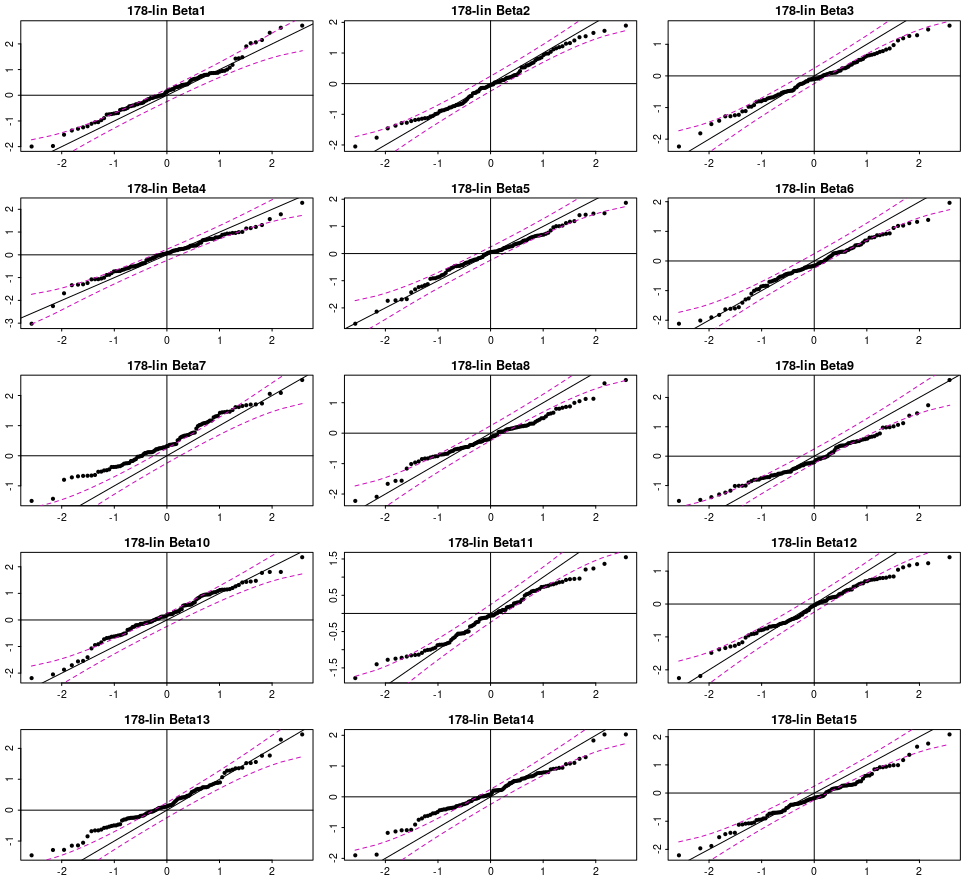
\includegraphics[width=.6\textwidth]{\fig/StR22-BetaHat-n100-d3-p5-parm1-nIS1000-lin-betaStat}
    \end{tabular}
  \end{tabular}

}


%====================================================================
\frame{\frametitle{Model 1: Composite likelihood} 

  \paragraph{The likelihood} is not the only admissible contrast for grounded statistical inference.

  \bigskip \bigskip \pause
  \paragraph{Composite likelihood} is one of the many others:
  \begin{itemize}
    \setlength{\itemsep}{1.25\baselineskip}
    \item build $B$ \emphase{overlapping} subsets of species, each with size $k$ (e.g. consider all pairs: $k=2$); 
    \item define the composite likelihood
    $$
    \cl_\theta(Y) = \sum_b \lambda_b \log p_\theta(Y^b); 
    $$
  \end{itemize}
  
  \bigskip \pause
  \paragraph{Guaranties}
  \begin{itemize}
    \setlength{\itemsep}{1.25\baselineskip}
    \item Under general conditions, $\widehat{\theta}_{CL} = \argmax_\theta \cl_\theta(Y)$ is consistent and asymptotically normal \refer{VRF11}.
    \item The (MC)EM algorithm can be adapted to the maximum composite likelihood estimation.
  \end{itemize}

}
